\documentclass[11pt,a4paper]{scrartcl}
\typearea{12}
\usepackage{graphicx}
\usepackage{pstricks}
\usepackage{listings}

\usepackage{tikz}
\usetikzlibrary{shapes, arrows.meta, positioning, shadows}
\usepackage{amsmath}



\tikzset{
    state/.style={
           rectangle,
           rounded corners,
           draw=black, very thick,
           inner sep=2pt,
           text centered,
           },
}
\tikzset{
    on/.style={
           circle,
           draw=red, very thick,
           inner sep=2pt,
           fill=red!25,
           },
}


\tikzset{
    off/.style={
           circle,
           draw=blue, very thick,
           inner sep=2pt,
           text centered,
           },
}



\lstset{language=python}
\pagestyle{headings}
\markright{PHPHM0017 - 3 modelling oscillations - Conor Houghton}

\begin{document}

\section*{Modelling oscillations}

So far we have looked at how to model individual neurons; here we will
consider how we can model the brain at a larger scale and, in
particular, we will look at models of neural oscillations. In fact, we
will look at two such models, the first is a model of two interacting
populations of neurons, a population of excitatory neurons interacting
with a population of inhibitory neurons. We will see that this system
oscillates. The second model is more abstract still, it takes the
oscillations as a fact that does not need to accounted for and models
different regions of the brain as different oscillators, looking to
examine how these interact.

All this will seem like a bit of jump, we go from looking at
individual neurons to whole groups of neurons without trying to show
in any detail how one leads to the other. There are two reasons for
this, the first is just brevity, it is possible to consider sequences
of approximations, assumptions and insights that leads from one scale
to the next, but that is a whole subject in itself. However, the
second reason is that the more principled approach, deriving the
equations for populations from the equations for simple neurons, is
very involved and complicated without always being rigorous, in other
words trying to do things too carefully can be very tricky but all you
really learn is that there are lots of approximations and guesses involved.

The idea, so, is to imagine the activity of lots of neurons, all with
their own internal voltage and other dynamical variables related to
ion concentrations and recent spiking, and to imagine the activity of
lots of synapses, with all the immense complexity that describes, to
imagine a whole plethora of variables changing according to different
differential equations, and to hope that taken at a large enough scale
and with enough tolerance for approximation and guess-work, it will be
possible to sort of average over all that's going on and to find a
handful of equations that captures enough of the behaviour to be
useful.

This idea is often called neural mass modelling and the models are
often called Wilson-Cowan models. This is something of a misnomer, the
original Wilson-Cowan model was very principled, deriving equations in
a careful mathematical way from the underlying neuronal dynamics. The
Wilson-Cowan equations are quite complicated and are often field
equations, which means they have variables for location as well as
time. However, generally, neural mass models do not have location
variables, instead, there is a single equation for a populations of a
particular type of neurons in some location, all the pyramidal cells
in CA3 for example. Often the equations called Wilson-Cowen equations
recognize that the complexity of neuronal dynamics is related to
synaptic dynamics, so they are careful to model the synapses in some
detail, even if the model is for the whole population of synapses;
this makes sense too because it is largely the synaptic current that
is detected by EEG. Here, however, we will look at models that appear
to ignore the synapse in favour of the neuron, in fact, we will be a
bit vague about what we are modelling, we will refer to `activity'
without really specifying what we mean. For convenience, it might
appear that activity means neuronal activity but there are other
interpretations of these equations though which link `activity' to
synapses. We will float above these concerns.

A neural mass model is a model of lots of neurons; we know that
signals travel from neuron to neuron in the form of spikes, but one of
the obvious approximations we make when dealing with neuronal
populations rather than individual neurons is to ignore the individual
spikes and track instead the firing rate, the rate spikes are being
produced across the neuronal population. 

In a neuron the relationship between input to the neuron and the
firing rate is not linear. Lets write
\begin{equation}
  r=f(y)
\end{equation}
where $r$ is the firing rate and $y$ is the input, or perhaps some
leaky integration of the recent input and $f$ is supposed to map from
one to the other. A first guess might be that $f(y)=ay+b$ would be a
good approximation for some constants $a$ and $b$. However, it is not!
Even for the leaky integrate-and-fire neurons we looks at, with
constant input, the relationship is not a straight line, see
Fig.~\ref{fig:fIcurve}; the relationship between firing rate and input
current is a commonly measured property of neurons, called the
fI-curve. In general real fI-curves share some of the features of the
fI-curve for leaky integrate-and-fire neurons in that the rate is
constant, perhaps zero or perhaps some small value, until there is a
sudden change to increasing $f$; it is common for the $f$ to rise
quickly before moderating its rise, however in real neurons it usually
levels off more than it does for the leaky integrate-and-fire neuron.

The fI-curve situation is intended to motivate the inclusion of
non-linearities in the model we will construct, a little thought might
make you think the non-linearities are in the wrong place. This is
related, as described, to a little vagueness as to what we are
actually modelling, so we are going to avoid worrying too much about the details!

\begin{figure}
  \begin{center}
  \includegraphics{fIcurve.png}
  \end{center}
  \caption{\textbf{The fI-curve for an integrate and fire
      neuron}. Here a leak integrate-and-fire neuron is simulated for
    10 seconds different values of $R_mI_e$, the number of spikes is
    counted and used to calculate a firing rate. This give the firing
    rate, in Hz, as a function of input current, while this is
    labelled $I$ here, for convenience this is actually $R_mI_e$ and
    is in mV. The other parameters, in the notation used in the
    previous notes, are $\tau_m=10$ ms, $V_T=-55$ mV an $E_l=V_R=-70$
    mV.}
  \label{fig:fIcurve}
\end{figure}

\subsection*{The pyramidal / inhibitory neurons circuit}

Here we will consider a neural mass model of the pyramidal-inhibitory
circuit. This circuit is a common leit-motif in discussions of neural
computation and has a tendency to generate oscillations. The neural
mass model we use is particularly simple and is described in a paper
by Onslow, Jones and Bogacz\footnote{Angela C. E. Onslow, Matthew
W. Jones, Rafal Bogacz (2014) A Canonical Circuit for Generating
Phase-Amplitude Coupling. PLoS One 9:e102591}. In the
pyramidal-inhibitory circuit the pyramidal neurons tend to signal to
each other as well as to the inhibitory cells, whereas the inhibitory
cells signal only to pyramidal cells, see Fig.~\ref{fig:circuit}.

\begin{figure}
  \begin{center}
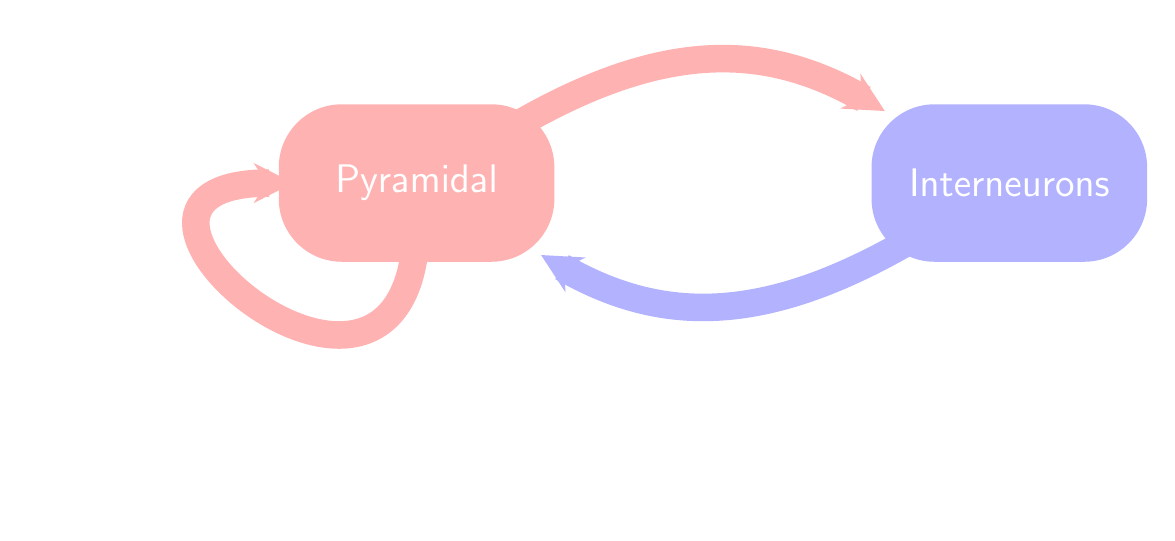
\begin{tikzpicture}[
    node distance=4cm,
    mynode/.style={
        thick, rectangle, rounded corners=8mm, minimum width=3.5cm, minimum height=2cm,
        font=\sffamily\Large, fill=#1, text=white
    },
    arrow/.style={
        -{Stealth[length=5mm, width=5mm]}, line width=3.5mm, draw=#1,
        shorten <=-5.5mm, shorten >=-2mm
    },
    selfloop/.style={
        looseness=5, out=270, in=180, distance=3cm
    }
]

% Nodes
\node[mynode=red!30] (pyramidal) {Pyramidal};
\node[mynode=blue!30, right=of pyramidal] (interneurons) {Interneurons};

% Arrows
\draw[arrow=red!30] (pyramidal) to[bend left] (interneurons);
\draw[arrow=blue!30] (interneurons) to[bend left] (pyramidal);
% Self-loop for Pyramidal node
\draw[arrow=red!30, selfloop] (pyramidal) to (pyramidal);

\end{tikzpicture}
  \end{center}
  \caption{\textbf{The pyramidal-interneuron circuit}. There are two
    populations, the pyramidal cells have recurrent connections as
    well as connections to the inhibitory cells, the inhibitory cells
    signal to the pyramidal cells.}
  \label{fig:circuit}
\end{figure}

In
the model there are activity levels for both the pyramidal neurons
($E$) and the inhibitory neurons ($I$), each satisfies a decay equation with some input. Hence for the pyramidal neurons
\begin{equation}
  \tau_E\frac{dE}{dt}=-E+f(\theta_{E}+w_{EE}E-w_{IE}I)
\end{equation}
where $\tau_E$ is a time scale, $\theta_E$ is an external input, $w_{EE}$ is coupling strength
for the recurrent connections and $w_{IE}$ is the strength of the
coupling from the inhibitory neurons to the pyramidal neurons. The inhibitory neurons satisfy a similar equation:
\begin{equation}
  \tau_I\frac{dE}{dt}=-I+f(\theta_{I}+w_{EI}E)
\end{equation}
with the obvious notation. The main difference, apart from swapping
$I$s and $E$s is that there is no recurrent connection. In both cases
the nonlinear function $f(\theta)$; this might be thought of as
translating between input and firing rate. For this model
$$f(\theta)=\frac{1}{1+\exp{[-\beta(\theta-1})]}$$ where $\beta$ is a
parameter. This function may seem like an odd choice since
$f(0)\not=0$, but it is convenient and $f(0)$ is very small; most
models go to some effort to avoid this anomaly but it is easier to
ignore it.

The behaviour of the model depends on the parameters, in the paper by
Onslow, Jones and Bogacz they suggest $\theta_E=0.5$, $\theta_I=0.0$;
$w_{EE}=2.4$, $w_{EI}=w_{IE}=2.0$ and $\tau_E=\tau_I=0.0032$ s. The
resulting dynamics is plotted in Fig.~\ref{fig:pi}\textbf{A}. Often when
studying dynamics it is informative to look at the phase diagram, this
means picking a variable, say $E$, and plotting it against its
derivative, this means looking at $(E,dE/dt)$, this is shown in
Fig.~\ref{fig:pi}\textbf{B}. Now we have the model we can study its
behaviour, for example, in Fig.~\ref{fig:theta} we look at how the
oscillations change as the input to the pyramidal neurons
change. Ultimately, if might like to measure some data and then fit
the model, or fit some more elaborate version of the model with
populations corresponding to different pyramidal-interneuron circuits
in different brain regions. Different parameters for the model when
fit to different subjects might offer some clue, in terms of
connectivity or other parameters, as to what creates a difference in
behaviour.


\begin{figure}
  \begin{center}
    \begin{tabular}{ll}
      \textbf{A}&\textbf{B}\\
  \includegraphics{pi.png}&  \includegraphics{phase.png}
\end{tabular}
    \end{center}
  \caption{\textbf{Oscillations}. The model is run for 500 ms with the
    parameters taken from the paper. In \textbf{A} the values of $E$
    and $I$ are plotted against time. After an initial higher peak it
    quickly settles into a regular oscillation close to 50 Hz.
    \textbf{B} shows the phase diagram. For each variable, $E$ and $I$
    is plotted against its derivative. In this way of looking at
    dynamics we lose any idea of how long things take, but it does
    show us what is going on, mathematicians have found that phase
    diagrams are very useful when studying how the behaviour of a
    dynamical system changes and its parameters are changed.}
  \label{fig:pi}
\end{figure}


\begin{figure}
  \begin{center}
  \includegraphics{theta.png}
  \end{center}
  \caption{\textbf{Changing input}. Here the model is run using the same parameters as elsewhere but with one exception, the value of the input $\theta_E$ is varied. For each value the model is run for 250 ms to let it settle down. Over the following 250 ms the minimum and maximum value of $E$ is found and plotted. If $\theta_E$ is near zero, or bigger than about 1.25 the maximum and minimum coincide, showing there is no oscillation.}
  \label{fig:pi}
\end{figure}





\end{document}
